\section{动机}
\label{sec:motivation}

\begin{frame}
  \begin{center}
    \Huge{\textcolor{red}{动机}}
  \end{center}
\end{frame}

\subsection{极限编程}

\begin{frame}{极限编程}
    \centering
    \begin{figure}
      \centering
      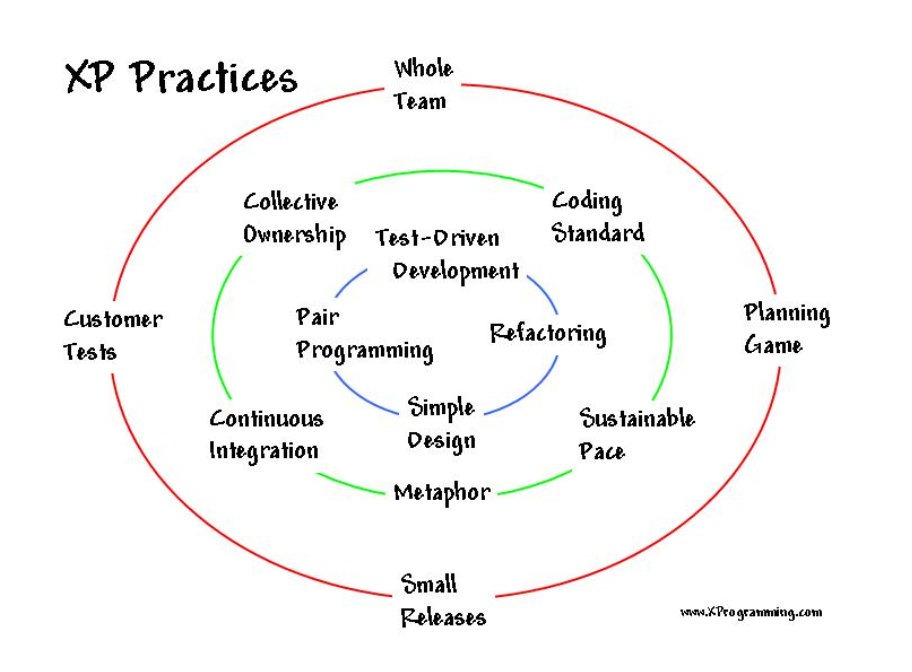
\includegraphics[width=0.8\textwidth]{xp-practices.png}
    \end{figure}
\end{frame}

\begin{frame}{测试 vs. TDD}
    \centering
    \begin{figure}
      \centering
      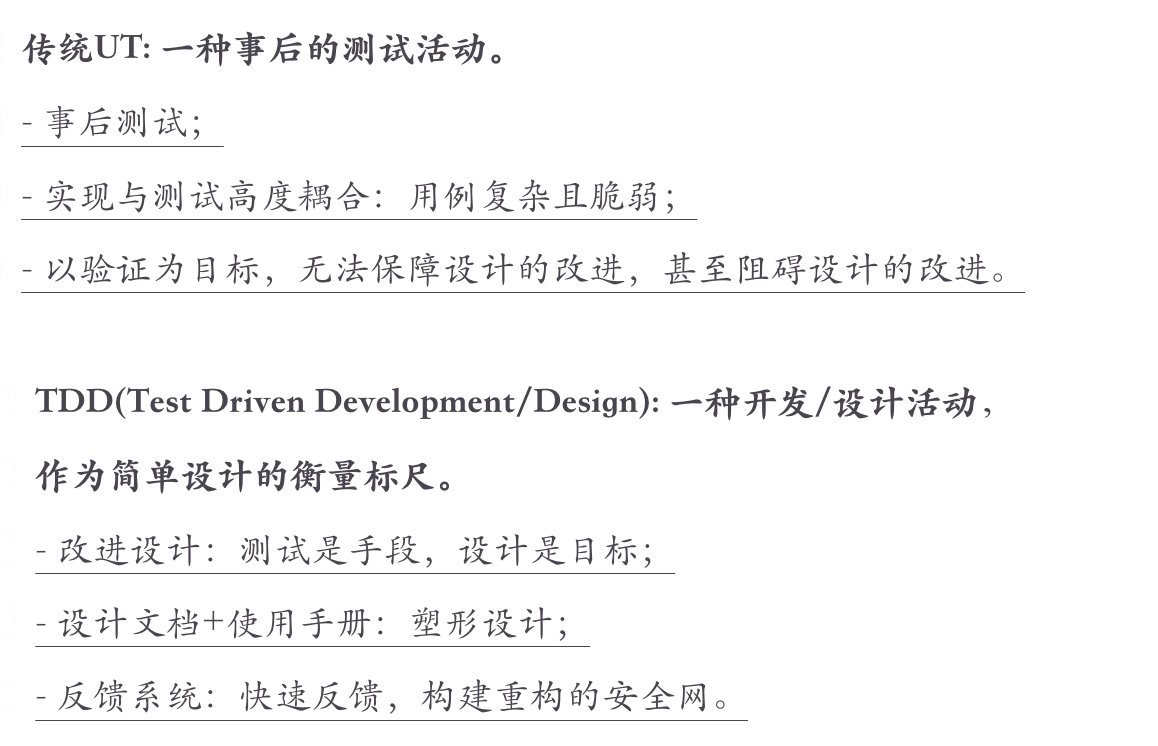
\includegraphics[width=0.8\textwidth]{tdd-test.png}
    \end{figure}
\end{frame}

\begin{frame}{xUnit实现模式}
    \centering
    \begin{figure}
      \centering
      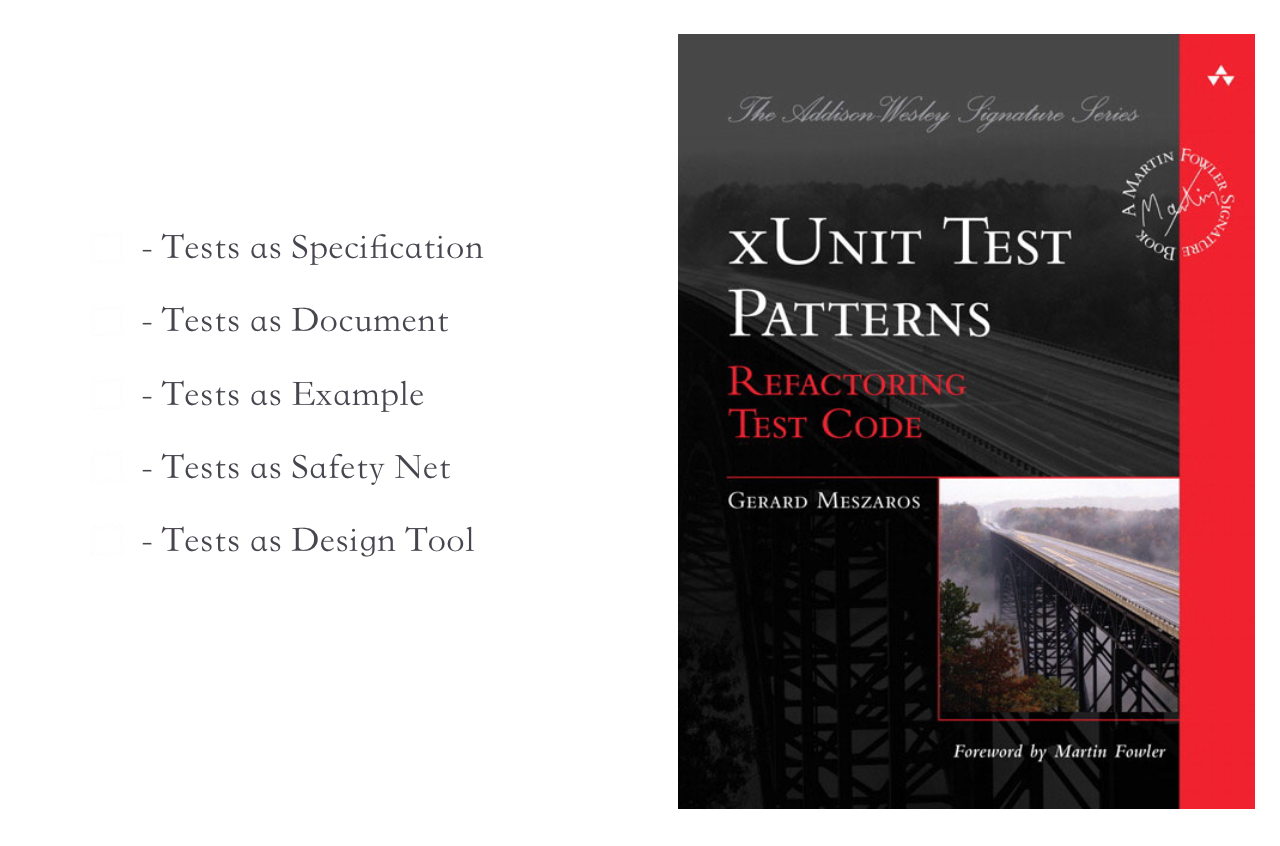
\includegraphics[width=0.8\textwidth]{xunit-patterns.png}
    \end{figure}
\end{frame}

\begin{frame}{回到主题:为什么需要一个全新的C/C++测试框架?}
  \begin{center}
    \LARGE{\textcolor{red}{让TDD和重构更高效,让编程添加更多乐趣}}
  \end{center}
\end{frame}

\begin{frame}{我的偏爱} 
  \begin{enumerate}
    \item \textcolor{red}{C/C++}: GoogleTest/Catch2
    \item \textcolor{red}{Java}: JUnit/Spock
    \item \textcolor{red}{Python}: unittest
    \item \textcolor{red}{Ruby}: RSpec
    \item \textcolor{red}{Scala:} ScalaTest
  \end{enumerate}
\end{frame}

\subsection{Google Test}

\begin{frame}{命名困难}
    \centering
    \begin{figure}
      \centering
      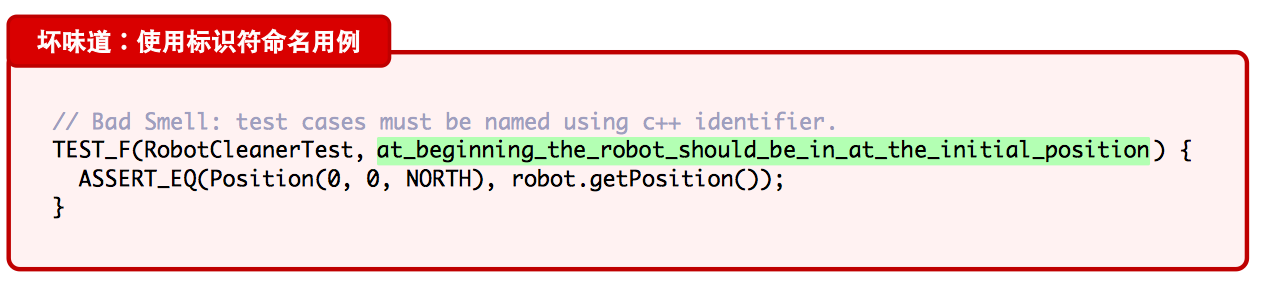
\includegraphics[width=1.0\textwidth]{gtest-bad-smell-1.png}
    \end{figure}
\end{frame}

\begin{frame}{重复设计}
    \centering
    \begin{figure}
      \centering
      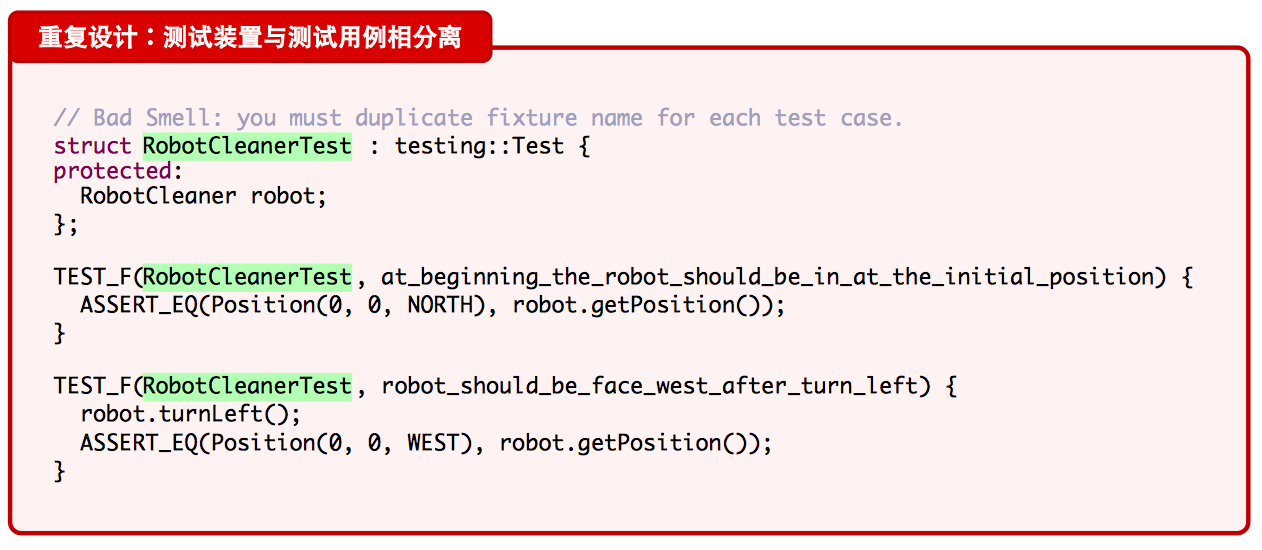
\includegraphics[width=1.0\textwidth]{gtest-bad-smell-2.png}
    \end{figure}
\end{frame}

\begin{frame}{隐式继承}
    \centering
    \begin{figure}
      \centering
      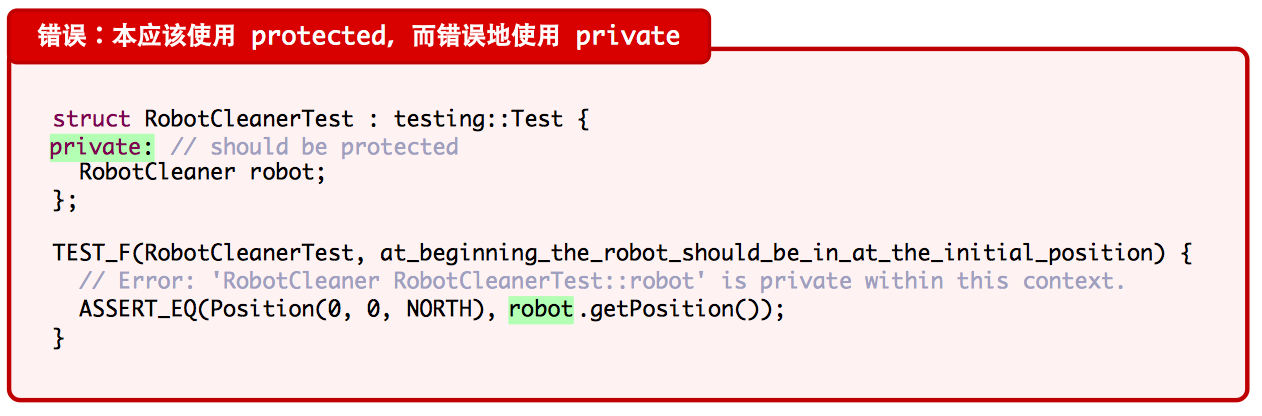
\includegraphics[width=1.0\textwidth]{gtest-bad-smell-3.png}
    \end{figure}
\end{frame}

\begin{frame}{易于误用1}
    \centering
    \begin{figure}
      \centering
      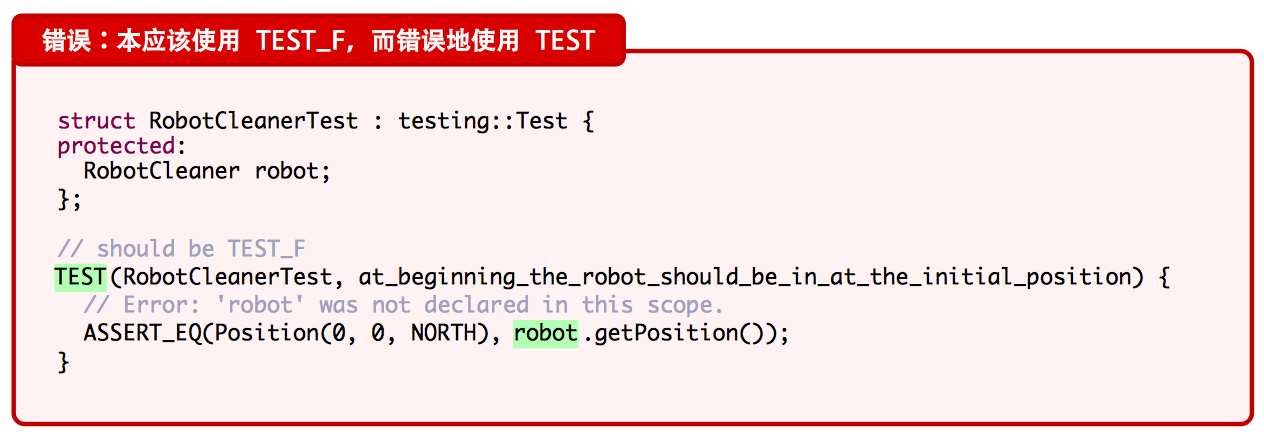
\includegraphics[width=1.0\textwidth]{gtest-bad-smell-4.png}
    \end{figure}
\end{frame}

\begin{frame}{易于误用2}
    \centering
    \begin{figure}
      \centering
      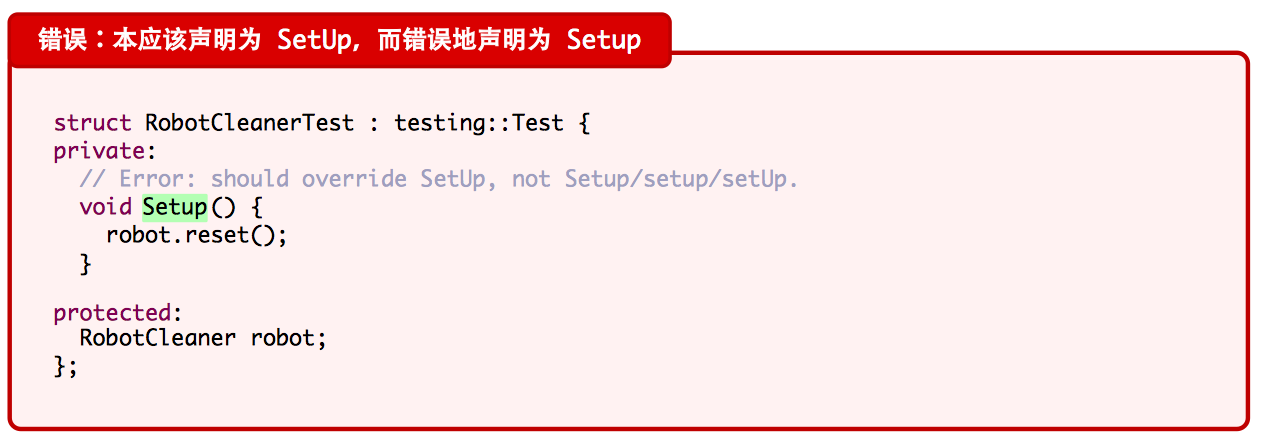
\includegraphics[width=1.0\textwidth]{gtest-bad-smell-5.png}
    \end{figure}
\end{frame}
